% ~~~ [ Code Coverage ] ~~~~~~~~~~~~~~~~~~~~~~~~~~~~~~~~~~~~~~~~~~~~~~~~~~~~~~~~

\subsubsection{Code Coverage}
\label{sec:ver_code_coverage}

Code coverage is a measurement for tracking what parts of the code that gets executed when running test cases. The Go project takes an interesting approach to tracking code coverage, which utilizes the production quality source code analysis and transformation libraries available in Go. Instead of generating platform-dependent assembly which tracks the execution of various branches, Go inject unique tracking statements on each line of the original source code. This approach is platform-independent by design, and may easily be extended to support heat maps which track how often each line gets executed \cite{go_cover}.

As the lexer of any language is a fundamental building block on which other libraries and components depend, the test cases of the LLVM IR lexer aimed for a 100\% code coverage of any code not related to input/output errors (e.g. ``file not found''); as illustrated in figure \ref{fig:lexer_code_coverage}. This rigorous testing uncovered several faulty assumptions in the lexing logic, which were later corrected.

\begin{figure}[htbp]
	\begin{center}
		\begin{verbatim}
$ go test -coverprofile=lexer.out github.com/llir/llvm/asm/lexer
$ go tool cover -func=lexer.out
llvm/asm/lexer/lexer.go:36:    ParseFile      80.0%
llvm/asm/lexer/lexer.go:118:   emit           100.0%
llvm/asm/lexer/lexer.go:139:   next           100.0%
llvm/asm/lexer/lexer.go:158:   accept         100.0%
llvm/asm/lexer/state.go:38:    lexToken       100.0%
llvm/asm/lexer/state.go:131:   lexComment     100.0%
…
llvm/asm/lexer/state.go:364:   lexQuote       100.0%
llvm/asm/lexer/state.go:585:   unescape       100.0%
total:                         (statements)   97.6%
		\end{verbatim}
		\caption{A summary of the code coverage for a selection of the LLVM IR lexer functions, as visualized by the \texttt{cover} tool.}
		\label{fig:lexer_code_coverage}
	\end{center}
\end{figure}

A breif summary of the code coverage for the various software artefacts is presented in figure \ref{tbl:code_coverage_summary}.

\begin{savenotes}
	\begin{table}[htbp]
		\begin{center}
			\begin{tabular}{|l|l|}
				\hline
				Code coverage & Component \\
				\hline
				97.6\% & LLVM IR lexer\footnote{As of Git revision \texttt{bbba2831ad079074516041907d16c347e388a310}} \\
				0.0\% & Control flow generation tool \\
				94.8\% & Subgraph isomorphism search library\footnote{As of Git revision \texttt{70967487ea73284c68a89e3fc566bc706603b6f7}} \\
				40.0\% & Control flow analysis tool\footnote{As of Git revision \texttt{019e846bc7058f8fb9f7517568505c96eeed97bf}} \\
				0.0\% & Code generation tool \\
				38.0\% & Post-processing tool\footnote{As of Git revision \texttt{02d38d1fbbf1c05bb11de89360a7cd8c38329a14}} \\
				\hline
			\end{tabular}
		\end{center}
		\caption{A summary of the code coverage of each component, presented roughly in the same order as they appear in the decompilation pipeline.}
		\label{tbl:code_coverage_summary}
	\end{table}
\end{savenotes}

Code coverage heat maps may be used to gain clarity in how often a line gets executed by the test cases. The use of heat maps were invaluable when stress testing the various prototypes of the subgraph isomorphism search algorithm, as they were able to identify several tricky corner cases; such as the ones illustrated in figure \ref{fig:iso_heat_map}

\begin{figure}[htbp]
	\begin{center}
		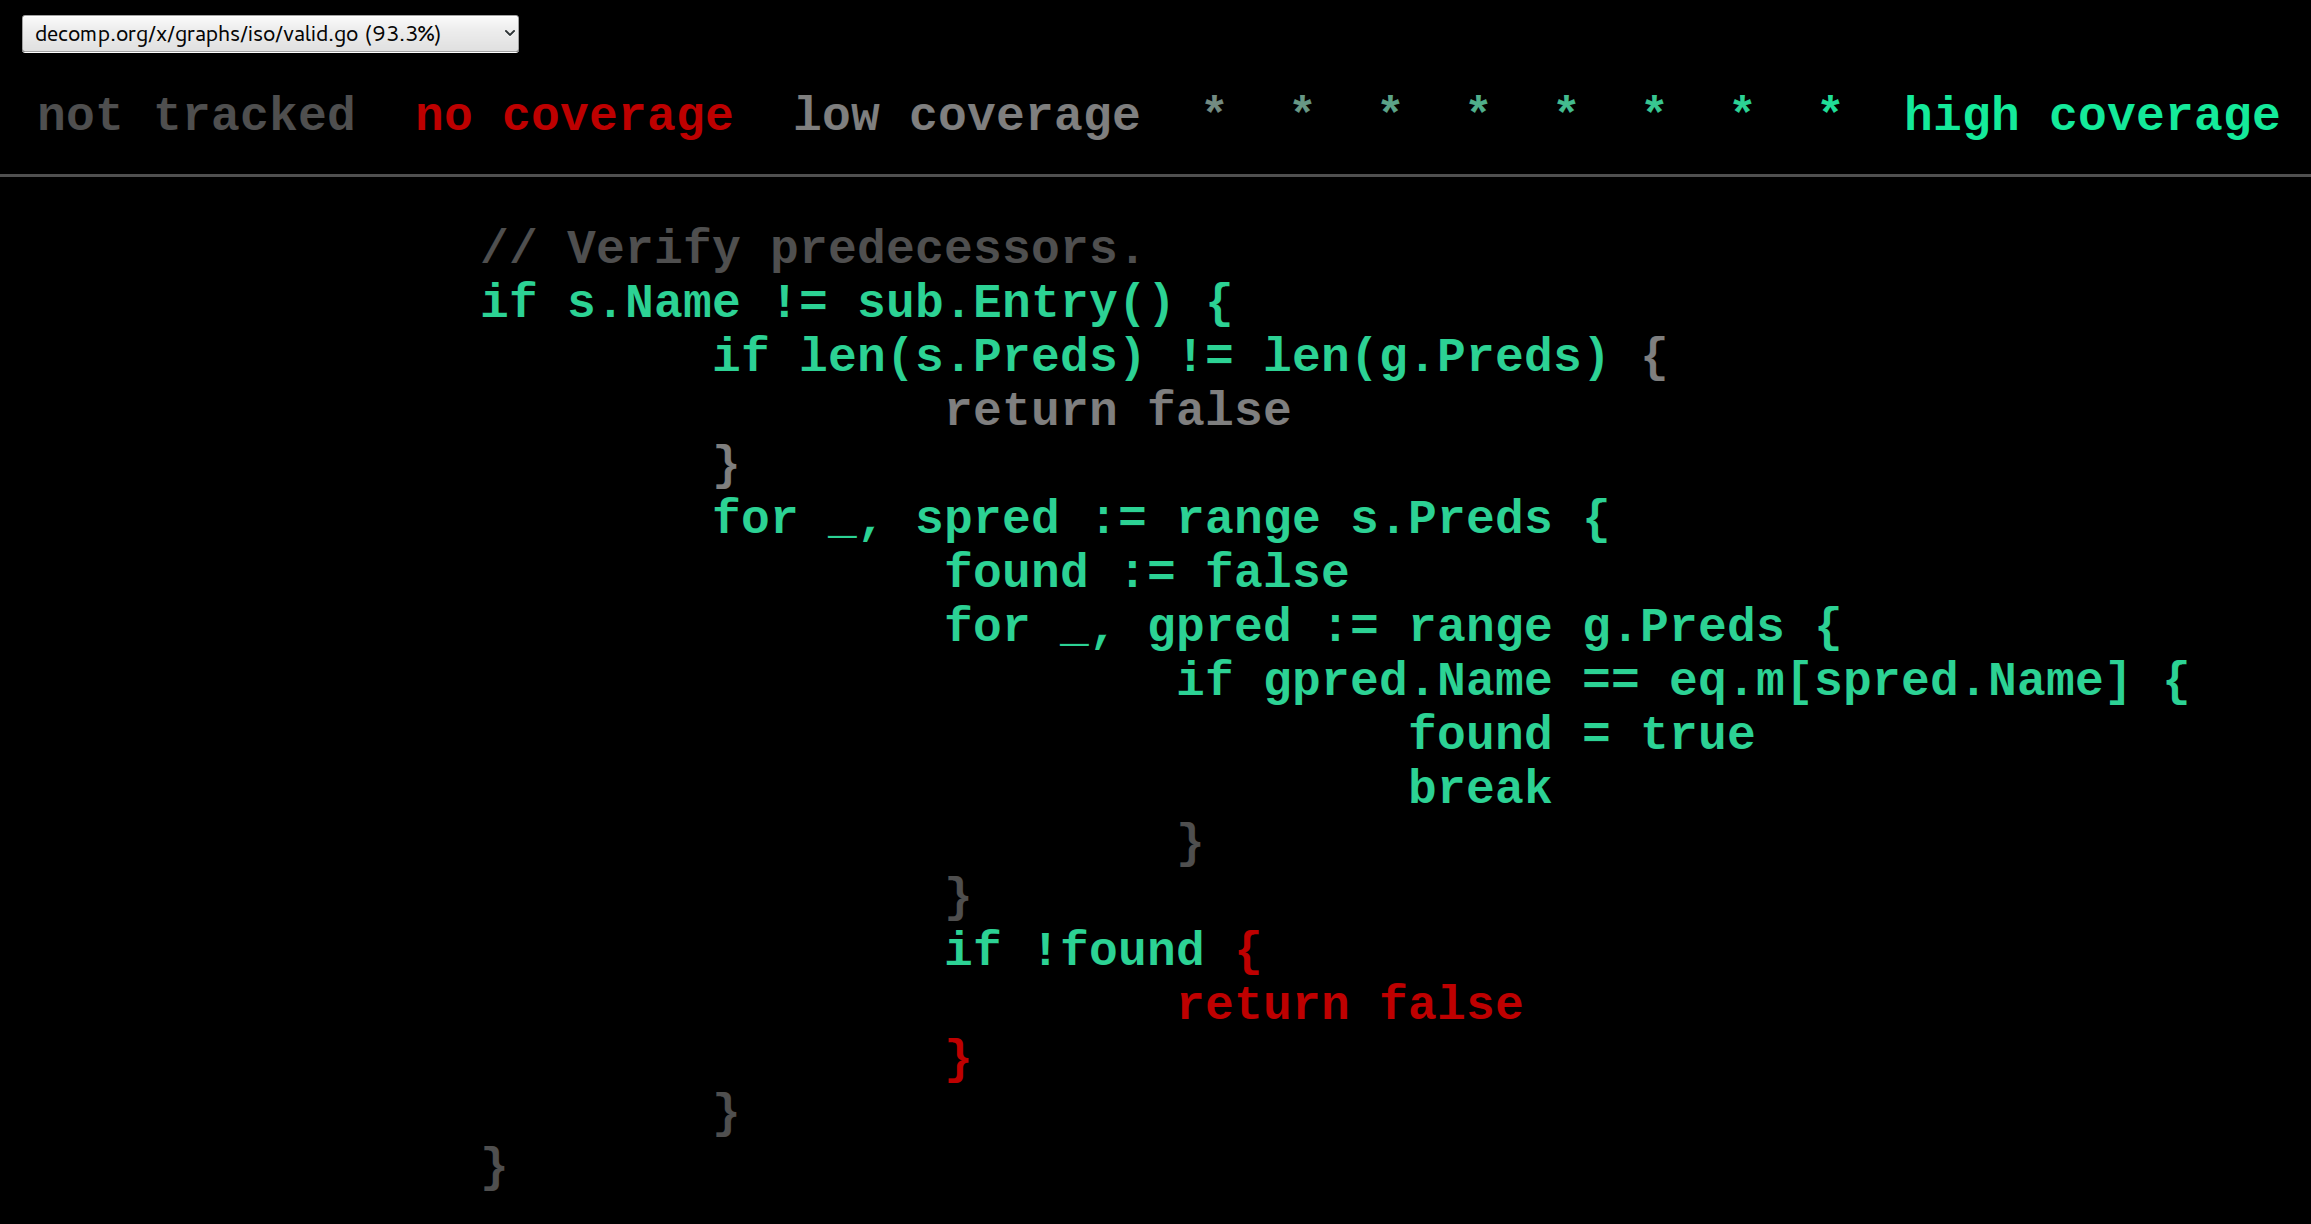
\includegraphics[width=\textwidth]{inc/8_ver/iso_heat_map.png}
		\caption{An extract from the code coverage heat maps of the subgraph isomorphism search algorithm, which has identified two corner cases that may require further validation. The first return statement is seldomly executed (as indicated by the \textit{gray} color), and the second return statement is never executed.}
		\label{fig:iso_heat_map}
	\end{center}
\end{figure}
